\documentclass[nobib, a4paper]{tufte-book}
\usepackage{microtype, ifluatex, ifxetex}
%Next block avoids bug, from  http://tex.stackexchange.com/a/200725/1913 
\ifx\ifxetex\ifluatex\else % if lua- or xelatex http://tex.stackexchange.com/a/140164/1913
  \usepackage{fontspec}
  \setmainfont[Renderer=Basic, Numbers=OldStyle, Scale = 1.0]{TeX Gyre Pagella}
  \setsansfont[Renderer=Basic, Scale=0.90]{TeX Gyre Heros}
  \setmonofont[Renderer=Basic]{TeX Gyre Cursor}

  \renewcommand{\textls}[2][5]{%
    \begingroup\addfontfeatures{LetterSpace=#1}#2\endgroup
  }
  \renewcommand{\allcapsspacing}[1]{\textls[15]{#1}}
  \renewcommand{\smallcapsspacing}[1]{\textls[10]{#1}}
  \renewcommand{\allcaps}[1]{\textls[15]{\MakeTextUppercase{#1}}}
  \renewcommand{\smallcaps}[1]{\smallcapsspacing{\scshape\MakeTextLowercase{#1}}}
  \renewcommand{\textsc}[1]{\smallcapsspacing{\textsmallcaps{#1}}}
\fi

\usepackage{graphicx} % allow embedded images
  \setkeys{Gin}{width=\linewidth,totalheight=\textheight,keepaspectratio}
  \graphicspath{{images/}} % set of paths to search for images
\usepackage{amsmath,amssymb,amsthm,amsfonts,ulem,tikz}  % extended mathematics
\usepackage{booktabs} % book-quality tables
\usepackage{units}    % non-stacked fractions and better unit spacing
\usepackage{multicol} % multiple column layout facilities
\usepackage{fancyvrb,xcolor} % extended verbatim environments
  \fvset{fontsize=\normalsize}% default font size for fancy-verbatim environments
\usepackage{tikz-cd,bbm,mathbbol}
\DeclareSymbolFontAlphabet{\mathbbl}{bbold} %let's you use \mathbbl{k} for a field k
\hypersetup{colorlinks} %puts color to hyperlinks
\setcounter{secnumdepth}{2} 
\usepackage{enumerate}
\usepackage{mathabx}
\usepackage{mathtools}
\usepackage{nccmath}
\usepackage[english]{babel}
\usepackage{hyperref}
\hypersetup{
    colorlinks=true,    
    urlcolor=Cerulean,
    linkcolor = ForestGreen,
}
\usepackage[toc]{appendix}

\newcounter{dummy} %so that \pageref works properly
\usepackage[absolute]{textpos}
\setlength{\TPHorizModule}{\paperwidth} \setlength{\TPVertModule}{\paperheight}


\usetikzlibrary{decorations.pathreplacing,} %for braces with itemize
\newcommand{\tikzmark}[1]{\tikz[baseline={(#1.base)},overlay,remember picture] \node[outer sep=0pt, inner sep=0pt] (#1) {\phantom{A}};}


% Standardize command font styles and environments
\newcommand{\doccmd}[1]{\texttt{\textbackslash#1}}% command name -- adds backslash automatically
\newcommand{\docopt}[1]{\ensuremath{\langle}\textrm{\textit{#1}}\ensuremath{\rangle}}% optional command argument
\newcommand{\docarg}[1]{\textrm{\textit{#1}}}% (required) command argument
\newcommand{\docenv}[1]{\textsf{#1}}% environment name
\newcommand{\docpkg}[1]{\texttt{#1}}% package name
\newcommand{\doccls}[1]{\texttt{#1}}% document class name
\newcommand{\docclsopt}[1]{\texttt{#1}}% document class option name
\newenvironment{docspec}{\begin{quote}\noindent}{\end{quote}}% command specification environment
\newcommand{\cat}[1]{{\normalfont\textsf{#1}}}
\DeclareMathOperator{\id}{id}
\newcommand{\adj}[4]{\begin{tikzcd}[ampersand replacement=\&, column sep=4ex]
					  	   #1 \colon #2	\ar[yshift=+.6ex]{r}
					  	\& #3 \colon #4	\ar[yshift=-.4ex]{l}
					 \end{tikzcd}}

\theoremstyle{plain}
\newtheorem{thm}{Theorem}[section]
\newtheorem{cor}[thm]{Corollary}
\newtheorem{prop}[thm]{Proposition}
\newtheorem{lem}[thm]{Lemma}

\theoremstyle{definition}
\newtheorem{defn}[thm]{Definition}
\newtheorem{conj}[thm]{Conjecture}

\theoremstyle{remark}
\newtheorem{ex}[thm]{Example}
\newtheorem{rmk}[thm]{Remark}
\newtheorem{ntn}[thm]{Notation}

\newtheorem{exe}[thm]{Exercise}
\newtheorem{prb}[thm]{Problem}

\usepackage[
    type={CC},
    modifier={by-nc-sa},
    version={4.0},
]{doclicense}

\usepackage{tcolorbox}

\usepackage[numbers, sort]{natbib}
\setlength{\bibsep}{3pt}
\renewcommand{\bibfont}{\small}
\usepackage{doi}

\newcommand{\cC}{\mathcal{C}}
\newcommand{\cE}{\mathcal{E}}
\newcommand{\cL}{\mathcal{L}}
\newcommand{\cO}{\mathcal{O}}
\newcommand{\cH}{\mathcal{H}}
\newcommand{\cI}{\mathcal{I}}
\newcommand{\cT}{\mathcal{T}}
\newcommand{\cB}{\mathcal{B}}
\newcommand{\cU}{\mathcal{U}}

%\newcommand{\bC}{\mathbb{C}}
\newcommand{\N}{\mathbb{N}}
\newcommand{\Z}{\mathbb{Z}}
\newcommand{\Q}{\mathbb{Q}}
\newcommand{\R}{\mathbb{R}}
\newcommand{\bS}{\mathbb{S}}
\newcommand{\bT}{\mathbb{T}}

\newcommand{\bx}{\bm{x}}
\newcommand{\bp}{\bm{p}}
\newcommand{\bv}{\bm{v}}

\let\d\relax
\DeclareMathOperator{\d}{d}
\DeclareMathOperator{\D}{D}
\DeclareMathOperator{\Id}{Id}
\DeclareMathOperator{\diag}{diag}
\let\mod\relax
\DeclareMathOperator{\mod}{mod}
\DeclareMathOperator{\curl}{curl}
\DeclareMathOperator{\Vol}{Vol}


\title{Analysis\\ \noindent
on\\ \noindent
Manifolds
}
\author{Marcello Seri}
\publisher{Bernoulli Institute\\ \noindent
A.Y. 2020--2021\\ \noindent 
\MakeLowercase{\texttt{m.seri@rug.nl}}
}

\begin{document}
\maketitlepage

\newpage

\begin{fullwidth}
    ~\vfill
    \thispagestyle{empty}
    \setlength{\parindent}{0pt}
    \setlength{\parskip}{\baselineskip}
    Copyright \copyright\ \the\year\ \thanklessauthor
    
    \par Version 0.1 -- \today

    \vfill
    \small{\doclicenseThis}
    
\end{fullwidth}
    
\pagenumbering{roman}
\tableofcontents
\cleardoublepage

\pagenumbering{arabic}
\chapter*{Introduction}
\addcontentsline{toc}{chapter}{Introduction}

At the voice \emph{Mathematical analysis}, our modern source of truth -- Wikipedia -- says

\begin{quotation}
  \emph{Mathematical analysis} is the branch of mathematics dealing with limits and related theories, such as differentiation, integration, measure, infinite series, and analytic functions.

  These theories are usually studied in the context of real and complex numbers and functions. Analysis evolved from calculus, which involves the elementary concepts and techniques of analysis. Analysis may be distinguished from geometry; however, it can be applied to any space of mathematical objects that has a definition of nearness (a topological space) or specific distances between objects (a metric space). 
\end{quotation}

\newthought{In this sense}, our course will focus on generalizing the concepts of differentiation, integration and, up to some extent, differential equations on spaces that are more general than the standard Euclidean space.

This said, the Euclidean space $\R^n$ is \emph{the} prototype of all manifolds: it won't just be our simplest example, we will see that locally every manifold looks like a Euclidean space.

Euclidean spaces, and the Riemannian charts that you encountered in the \href{http://www.rolandvdv.nl/G20/}{Geometry course}, have a very strong property: they can be described with a set of \emph{global} coordinates.
Even though this means that all computations are explicit, it does make it harder to distinguish \emph{intrinsic}\footnote{I.e. independent from the choice of coordinates.} concepts.
Manifolds will force our hand to work in a \emph{coordinate-free} setting.
We will see that this will unleash a surprising power that will allow us to lay the foundation for a lot of the mathematics that will come in the rest of the curriculum.

These notes will focus on fundamental methods of differential geometry, in particular we will discuss manifolds, differential forms, integration, geometry of submanifolds, real and complex vector bundles, connections.
Throughout the course and the text, I will try to give particular emphasis on the usefulness of these topics in the mathematical theories of classical and quantum mechanics.

If the time permits it, we will give a brief tour of Riemannian metrics and the notion of curvature or of distributions and Frobenius theorem, depending on the preferences expressed in class.
This part of the material will not necessarily be part of the lecture notes\footnote{I will update this paragraph, if needed, in due course.}.

The course relies \emph{heavily} on your knowledge of linear and multilinear algebra, multivariable analysis\footnote{Make sure to review the material of \href{http://www.rolandvdv.nl/M19/}{Multivariable Analysis} before the course begins} and dynamical systems.
This should not come as a surprise: differential geometry and classical mechanics were born together as unique discipline, part of mathematical physics, before the various communities started diverging on their own paths.

An old mathematical joke says that
\begin{quote}
  differential geometry is the study of properties that are invariant under change of notation.
\end{quote}
Sadly, this is \emph{funny because it is alarmingly close to the truth}\footnote{Cit. Lee \cite{book:lee}.}
You will soon see that different references use different notations. I'll try to stick to the ones you used in the past courses when possible, falling back to \cite{book:lee} and \cite{book:tu} and to my personal preference when the latter disagree.

\marginnote{In addition to the reference books, these lecture notes have found deep inspiration from \cite{lectures:merry} and \cite{lectures:hitchin} (both freely downloadable from the authors websites), and from the advanced book \cite{book:abrahammarsdenratiu}.}
\newthought{These lecture notes} are by no means comprehensive.
In addition to the course recommended textbook \cite{book:tu}, you can refer to \cite{book:lee}: it is an incredibly good textbook and contains all the material of the course and much more.
I have requested for \cite{book:tu} book to be freely available via SpringerLink using the university proxy but this will take some time to become active.
However, you can already freely access Lee's book via the University proxy on \href{https://link.springer.com/book/10.1007/978-1-4419-9982-5}{SpringerLink} and it will provide a very good and extensive reference for this and other future courses.

The idea for the cut that I want to give to this course, came from the online \href{https://www.video.uni-erlangen.de/course/id/242}{Lectures on the Geometric Anatomy of Theoretical Physics} by Frederic Schuller and by the lecture notes of Stefan Teufel's Classical Mechanics course \cite{lectures:teufel} (in German).
In some sense I would like this course to provide the introduction to analysis and geometry that I whish was there when I prepared my \href{https://www.mseri.me/lecture-notes-hamiltonian-mechanics/}{first edition} of the Hamiltonian mechanics course.

\mainmatter

\chapter*{Einstein summation convention}
\addcontentsline{toc}{chapter}{Einstein summation convention}

As will become clear soon, sums of the type $\sum_i x^i e_i$ are unavoidably appearing all over the place when working on manifolds.
Therefore, throughout these notes we will apply the \emph{Einstein summation convention}: if the same index\footnote{For example, $i$ in the summation $\sum_i x^i e_i$.} appears exactly twice in a monomial term, once in the lower and once in the upper index position, then that term is understood to be summed over all possible values of that index\footnote{Usually from $1$ to the dimension of the space in question.}.

For instance, the expression
\begin{equation}
  a^{ij}b_l^k e_i e_k
\end{equation}
is a shorthand for
\begin{equation}
  \sum_{i,k} a^{ij}b_l^k e_i e_k.
\end{equation}

In general, we will use lower indices for basis of vector spaces\footnote{E.g., $(e_1,\ldots,e_n)$ will be the standard basis of $\R^n$.}, and upper indices for the components of a vector with respect to a basis\footnote{E.g., the $i$th-coordinate $x^i$ of $x\in\R^n$.}.
\marginnote[10pt]{Since the coordinates of a point $x\in\R^n$ are also its components with respect to the standard basis $(e_1, \ldots, e_n)$, for consistency they will be denoted $(x^1, \ldots, x^n)$ with upper indices.}

\chapter{Manifolds}\label{ch:manifolds}

\newthought{In the first two years} of your mathematical education, you have become familiar with calculus for functions and vector fields on $\R^n$.
As I mentioned in the introduction, euclidean spaces will be our prototypical example.
However, the generalization of calculus to curved spaces will require us to carefully isolate the mathematical structures associated to the various concepts.
This process will help us to discover the rich geometric structure that lies at the root of derivation and integration, which ultimately is of great mathematical interest and has revolutionized mathematical physics.

If you think carefully, this abstraction step was already in the air. Think about the concept of continuity.

\begin{enumerate}[a)]
  \item (High school) A function $f:\R\to\R$ is \emph{continuous} if you can draw it without lifting your pen from the page.
  Then, the derivative $f'(x)$ of $f$ at a point $x$ is just the slope of the function $f$ at the point $x$.
  
  \item (Analysis) A function is continuous if its left and right limits at each point exist and have the same value.
  Then, $f:\R\to\R$ is \emph{differentiable} at a point $x$ if the limit
  \begin{equation}
    f'(x) := \lim_{h\to0} \frac{f(x+h) - f(x)}{h} 
  \end{equation}
  exists, and is \emph{continuously differentiable} if $x\mapsto f'(x)$ is itself a continuous function.
  
  \item (Multivariable analysis) You generalized the concepts to functions with more than one variable.
  Continuity is practically unchanged but, now, a continuous function $f=(f^1, \ldots, f^m):\R^n\to\R^m$ is differentiable at $x=(x^1,\ldots,x^m)\in\R^n$ if there is a \emph{linear map}\footnote{That is, $T$ is a $m\times n$ matrix.} $T: \R^n\to\R^m$ such that
  \begin{equation}\label{eq:diff}
    \lim_{\|h\|\to 0} \frac{\|f(x+h) - f(x) - T h\|}{\|h\|} = 0.
  \end{equation}
  The map $Df(x) := T$ is the differential of $f$ and is nothing else than the Jacobian matrix of $f$ at the point $x$, that is
  \begin{equation}
    Df(x) = \begin{pmatrix}
      \frac{\partial f^1}{\partial x^1}(x) & \cdots & \frac{\partial f^1}{\partial x^n}(x) \\
      \vdots & \ddots & \vdots \\
      \frac{\partial f^m}{\partial x^1}(x) & \cdots & \frac{\partial f^m}{\partial x^n}(x) \\
    \end{pmatrix}.
  \end{equation} 
  The notion of continuous differentiability is unchanged\footnote{Note how the spaces are changing though: since it takes values in the space of $m\times n$ matrices, the differential $x\mapsto Df(x)$ is in fact a mapping of $\R^n \to \R^{mn}$.}, and in fact for $m=n=1$ it coincides with the one you gave for real functions.
  
  \item (Metric and topological spaces) A map $f:X\to Y$ between \emph{topological spaces} is continuous if preimages of open sets under $f$ are open. More explicitly, $f$ is continuous if for every open set $O\subset Y$, $f^{-1}(O)\subset X$ is an open set.

  If $X$ and $Y$ are \emph{metric spaces}, then this reduces to the definition given above.
  But how can we make sense of differentiability in this case? 
  
  If you have taken a course on calculus of variations, you know that you can make sense of \eqref{eq:diff} and give a notion of differentiability in the case $X$ and $Y$ are Banach spaces\footnote{Complete normed vector spaces.}.
  In general, a topological space is \emph{not} a vector space: there is no notion of adding points, least of all one of linearity.
\end{enumerate}

This is where differential geometry comes into play.
The rest of this chapter will be devoted to the introduction of \emph{smooth manifolds}, which are a class of topological spaces on which it is possible to make sense of the notion of differentiation even though they are not necessarily vector spaces.
We will do this in two stages.
First we will introduce \emph{topological manifolds}, which are topological spaces that \emph{locally} look like euclidean spaces.
Then we will endow topological manifolds with a so-called \emph{smooth structure}.
This will allow us to define differentiability and \emph{smooth manifolds}\footnote{These will just be topological manifolds with a smooth structure.}.

Without further ado, let's get started.

\subsection{Topological manifolds}

Since to speak of continuity we need topological spaces, it may be a good idea to remind you what they are and set some notation.
I will be very brief: if you need a more extensive reminder, you can refer to Appendix A of either \cite{book:tu} or \cite{book:lee}.

\begin{defn}
  Let $M$ be some set and $\cT$ a set of subsets of $M$.
  A pair $(M, \cT)$ is a \emph{topological space}\footnote{In such case the elements $O\in\cT$ of $\cT$ are all subsets of $M$ called \emph{open} subsets and $\cT$ is a topology on $X$.} if
  \begin{enumerate}[(i)]
    \item $M$ and $\emptyset$ are open, i.e., $M\in \cT$ and $\emptyset\in\cT$;
    \item arbitrary unions of families of open subsets are open;
    \item the intersection of finitely many\footnote{It is equivalent to require the intersection of any two open subsets to be open. (Why?)} open subsets is open.
  \end{enumerate}
\end{defn}

With topological spaces at hand, we can give a definition of continuity and introduce a way to compare topological spaces.

\begin{defn}
  A map $f: X \to Y$ between two topological spaces $(X,\cT)$ and $(Y, \cU)$ is called:
  \begin{itemize}
    \item \emph{continuous} if $U\in\cU$ implies that $f^{-1}(U)\in\cT$, that is, preimages of open sets under $f$ are open;
    \item \emph{homeomorphism} if it is bijective\footnote{I.e., one-to-one.} and continuous with continuous inverse.\marginnote{The existence of an homeomorphism between two spaces can be thought as those spaces being equivalent in a loose sense: they can be deformed continuously into each other.}
  \end{itemize}
\end{defn}

\begin{marginfigure}
  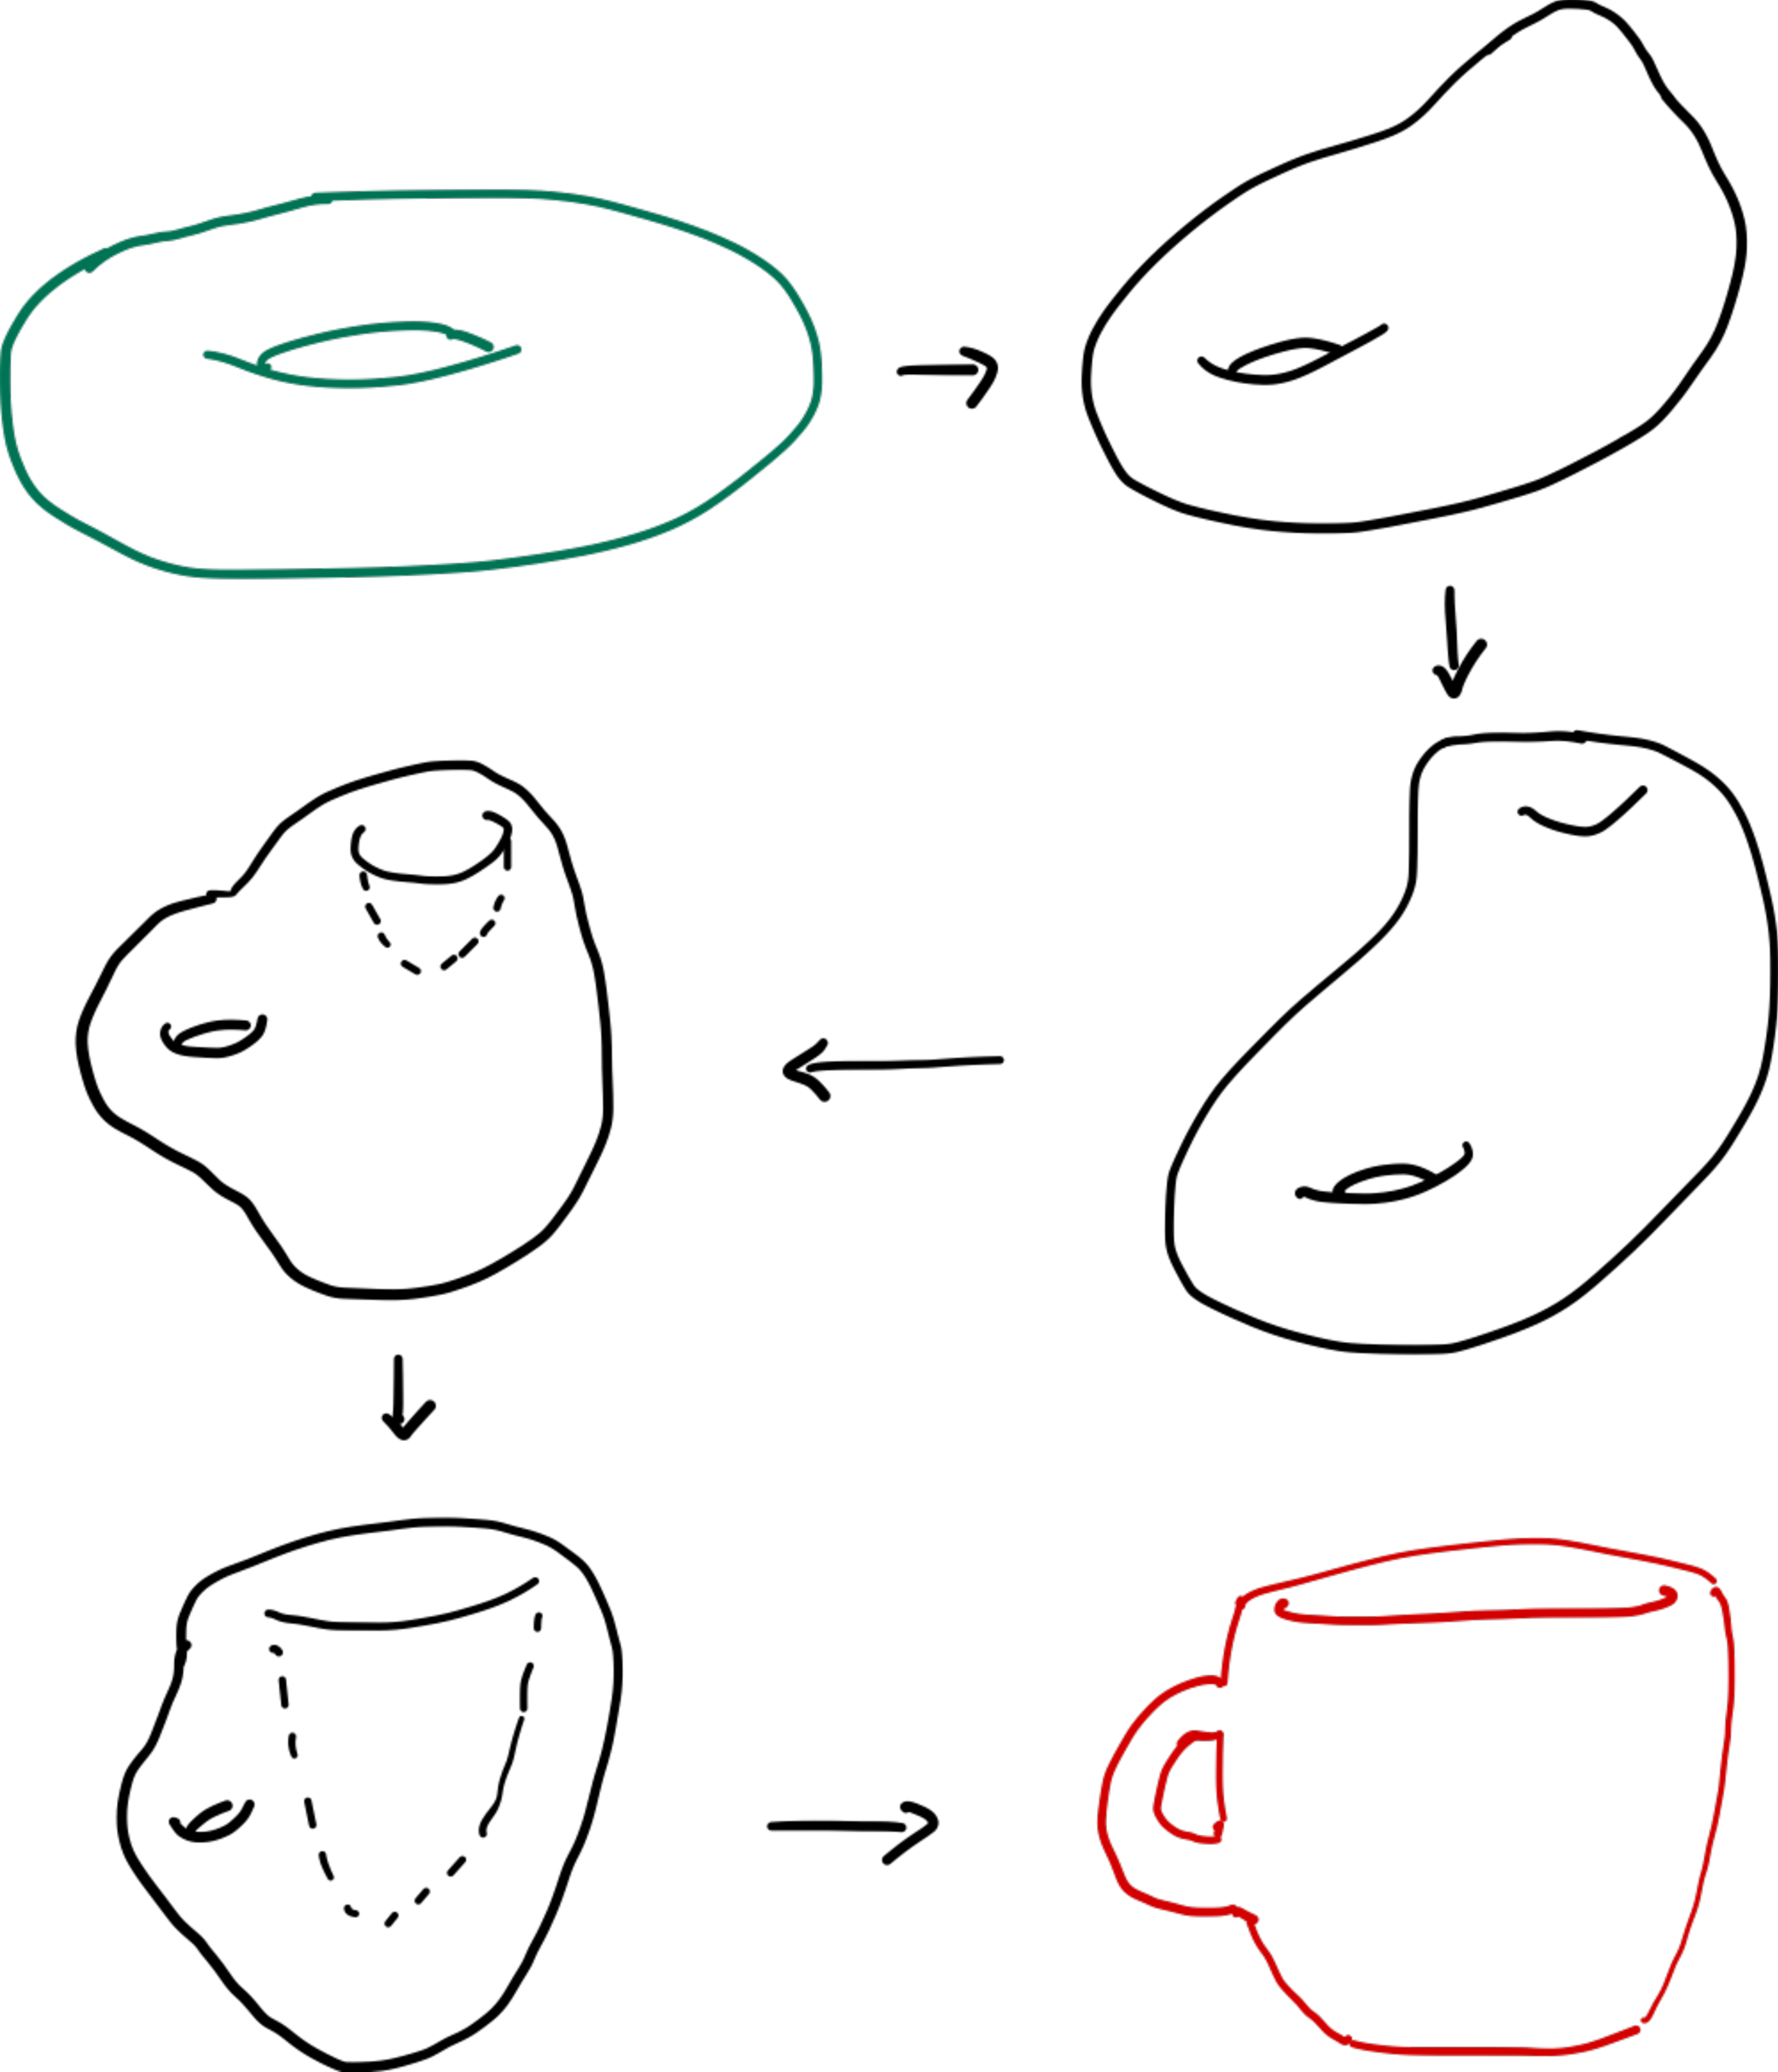
\includegraphics{images/1_1-dount-to-cup.pdf}
  \vspace{5pt}
\end{marginfigure}

\begin{defn}
  A topological space $(X, \cT)$ is \emph{Hausdorff} if every two distinct points admit disjoint open neighborhoods. That is, for every pair $x\neq y$ of points in $X$, there exist open subsets $O_x, O_y\in\cT$ such that $x\in O_x$, $y\in O_y$ and $O_x \cap O_y = \emptyset$.
\end{defn}

Topological spaces are extremely general, as such they may have very inconvenient -- someone would say nasty -- properties.
You can see this for yourself with the following exercise.

\begin{exe}
Let $X$ be an arbitrary set. Show that $\cT:=\{\emptyset, X\}$ defines a topology on $X$, called the \emph{trivial topology}. Show that on $(X, \cT)$ any sequence in $X$ converges to every point of $X$, and every map from a topological space into $X$ is continuous.
\end{exe}

Hausdorff spaces are still rather general: in particular, any metric space with the metric topology\footnote{Recall that in a metric space $X$ the \emph{metric topology} is defined in the following way: a set $U\subset X$ is called open if for any $x\in U$ there exists $\epsilon>0$ such that $U$ fully contains the ball of radius $\epsilon$ around $x$.} is Hausdorff.

\begin{defn}
  A topological space $(X, \cT)$ is \emph{second countable} if there exists a countable set $\cB\subset\cT$ such that any open set can be written as a union of sets in $\cB$.
  In such case, $\cB$ is called a (countable) basis for the topology $\cT$.
\end{defn}

\begin{exe}[Euclidean space $\R^n$]\label{exe:rntopsp}
  Let's consider on $\R^n$ the metric topology\footnote{See comment above.} induced by the Euclidean metric $d: \R^n \times \R^n \to [0, +\infty)$, $d(x,y) := \sqrt{\sum_{i=1}^n (x^i-y^i)^2}$.
  The topological space defined on $\R^n$ is Hausdorff and second countable.
\end{exe}

\begin{defn}[Topological manifold]
  A topological space\footnote{From now on, if we say that $X$ is a topological space we are implying that there is a topology $\cT$ defined on $X$.} $M$ is a \emph{topological manifold} of dimension $n$, or topological $n$-manifold, if it has the following properties
  \begin{enumerate}[(i)]
    \item $M$ is a Hausdorff space;
    \item $M$ is second countable;
    \item $M$ is \emph{locally euclidean} of dimension $n$, \marginnote{This means that any point $x\in M$ has a neighborhood that is homeomorphic to an open subset of $\R^n$.}that is, for any point $x\in M$ there exist an open subset $U\subset M$ with $x\in U$, and open subset $V\in\R^n$ and a homeomorphism $\phi: U\to V$.
  \end{enumerate}
\end{defn}

\begin{ntn}
  Reusing the notation of the definition above, we call \emph{(coordinate) chart} the pair $(U, \phi)$ of a \emph{coordinate neighborhood} $U$ and an associated \emph{coordinate map}\footnote{Or \emph{coordinate system}.} $\phi: U\to V$ onto an open subset $U=\phi(V)\subseteq\R^n$ of $\R^n$.
  Furthermore, we say that a chart is \emph{centered at $m\in U$} if $\phi(m) = 0$.
\end{ntn}

Don't get scared by the first two conditions: they are only needed to make sure that there are not too few open sets (Hausdorff) and not too many (second countable).

Be patient, we will soon see plenty of nontrivial examples.

\section{Differentiable manifolds}

The third property is the key for everything that will follow.
Since differentiability is a \emph{local} property and topological manifolds are \emph{locally} like euclidean spaces, we can lift the definitions directly from $\R^n$.



To do that, we 



\chapter{Differential Forms}

\chapter{Stokes' Theorem}

\chapter{de Rahm cohomology or fiber bundles}

\begin{appendices}
  \chapter{Solution to selected exercises}
  \section{Chapter \ref{ch:manifolds}}
  
  \newthought{Exercise \ref{exe:rntopsp}.}
  \begin{enumerate}
    \item[] Hausdorff. For $x\neq y\in\R^n$, let $\epsilon = d(x,y)/3$.
    Then the two balls $B_x(\epsilon) := \{z\in X \;\mid\; d(z,x)<\epsilon\}$ and $B_y(\epsilon)$ are disjoint open sets containing $x$ and $y$ respectively.
    \item[] Second countable. As countable basis for the topology we can take the open balls $B_\epsilon(x)$ with rational radii $\epsilon\in\Q$ and centers $x\in\Q^n$.
  \end{enumerate}
  
\end{appendices}

\bibliographystyle{plainnat}
\bibliography{aom}
\addcontentsline{toc}{chapter}{Bibliography}
\end{document}